\DiaryEntry{Advent of Code 2019, Day 10 - Interesting Stuff}{2020-08-26}{Maths}

The Advent of Code 2019, Day 10 challenge contains some inteestign questions this entry deals with.

\subsection{atan2 Function}

In one of the tasks it is necessary to calculate the angle of a line (between the zero-point and a point $P$) and the x-axis. The point $P_1$ has coordinates $x, y$ and the tangens is defined as

\bee
\tan \alpha = \frac{y}{x}
\eee

This is shown in the following Figure.

\begin{figure}[H]
\centering
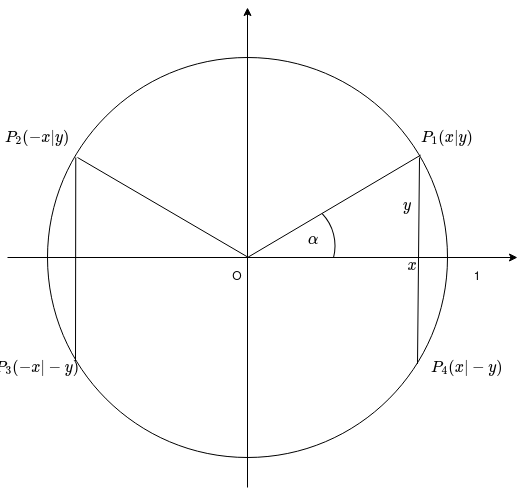
\includegraphics[scale=0.45]{images/AoC_2019_10_02.png}
\end{figure}

The following plot shows the tangens as function of the angle $\alpha$.

\begin{figure}[H]
\centering
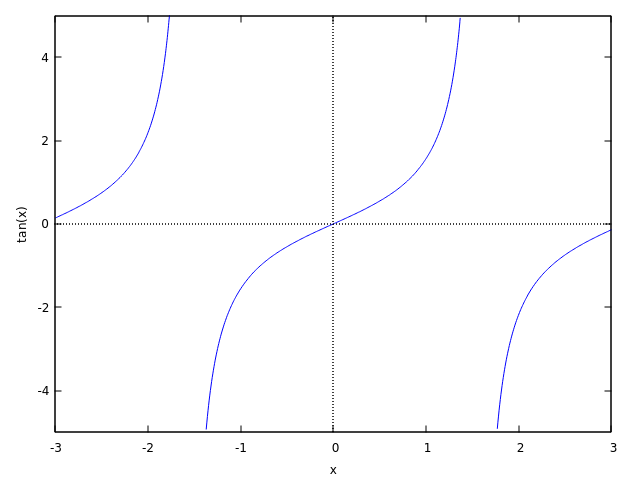
\includegraphics[scale=0.7]{images/AoC_2019_10_01.png}
\end{figure}

We are interested in obtaining the angle $\alpha$ of a given point $P$. The straightforward solution would be to use the $\arctan$ function; i.e.

\bee
\alpha = \arctan \frac{y}{x}
\eee

However, things are not that easy. In the division, the information about the sign is lost: If $x, y > 0$, the fraction $\frac{y}{x}$ has the same value as when both $x, y$ are negative and each has the same value. This second point (which yields the same value of $\frac{y}{x}$) is denoted as $P_3$. In a similar spirit, the points $P_2$ and $P_4$ yield the same value of the fraction.

The solution is the \emph{atan2} function, which does not take $\frac{y}{x}$ as argument, but the values $x, y$ \emph{separately}. This allows a clear separation of $P_1, P_3$ and $P_2, P_4$, respectively.

Because of periodic form of the $\tan$ function, it is not uniquely invertible; we have to restrict to a certain range. If we restrict the range to $(- \pi, \pi]$, the definition takes the following form.

\bee
\atantwo(y,x) = \begin{cases} \arctan \frac{y}{x} & x > 0 \\
  \arctan \frac{y}{x} + \pi & x < 0, y \geq 0 \\
  \arctan \frac{y}{x} - \pi & x < 0, y < 0 \\
  \frac{\pi}{2} & x=0, y > 0 \\
  -\frac{\pi}{2} & x=0, y < 0  
\end{cases}
\eee

From this we can see the follwing: If the point $P$ is in the right half-plane, we use the $\arctan$ function unchanged. The output of $\arctan$ is in $[-\pi/2, \pi/2]$, so we cover this range. If $P$ is in the second quadrant (i.e. $x < 0, y \geq 0$), we add $\pi$ to the result of $\arctan$. The range is therefore $[\pi/2, \pi]$. Finally, if $P$ is in the third quadrant (i.e. $x, y < 0$), then we subtract $\pi$ from $\arctan$ and the range is therefore $[-\pi, -\pi/2]$.


\subsection{Grid Points and Angle}

Suppose we now have a grid of integer points in the first quadrant; formally defined as $S = \{ (p,q) | p,q \in \{1,2,3,\ldots\} \}$. Let's now order these points by their angle $\alpha$ (as defined in the first Figure). The following Figure shows the points and their ordering.


\begin{figure}[H]
\centering
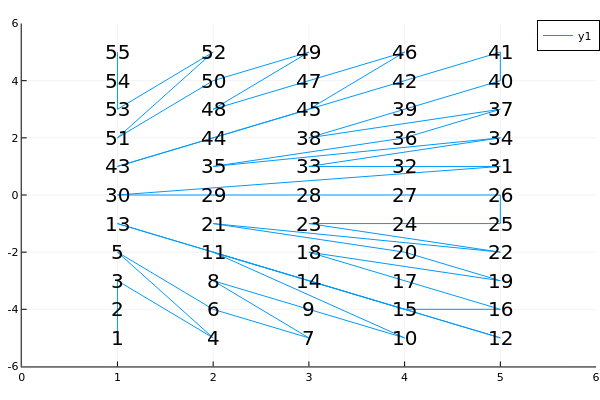
\includegraphics[scale=0.5]{images/AoC_2019_10_03.png}
\end{figure}

Along the $45°$ line the ordering is not consistent (Points $11 - 15$); however, there does not seem to be much order ansd the plot is also not symmetric along the $y = x$ line.

If we increase the number of points, we obtain the following Figure.

\begin{figure}[H]
\centering
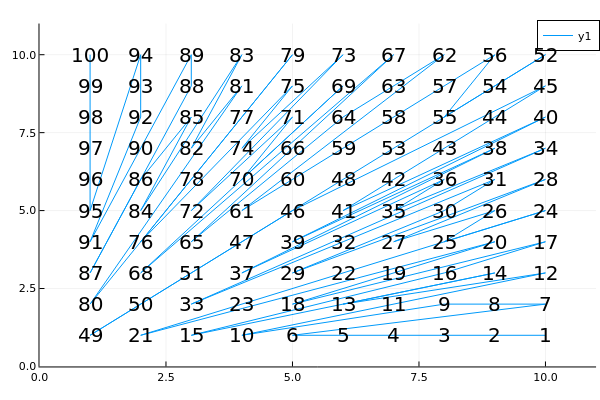
\includegraphics[scale=0.5]{images/AoC_2019_10_04.png}
\end{figure}



%%% Local Variables:
%%% mode: latex
%%% TeX-master: "journal"
%%% End:
